\documentclass[oneside,a4paper,14pt]{extarticle}
\usepackage[a4paper,letterpaper,top=20mm,bottom=20mm,left=20mm,right=10mm]{geometry}
\usepackage[russian]{babel}
\usepackage{indentfirst}
\usepackage{graphicx}
\usepackage{caption}
\usepackage{titlesec}
\usepackage{minted, fancyvrb}
\usepackage{hyperref}
\usepackage{enumitem}

% Форматирование заголовков
\titleformat{\section}{\normalsize\bfseries}{\thesection}{1em}{}
\titleformat{\subsection}{\normalsize\bfseries}{\thesubsection}{1em}{}
\titleformat{\subsubsection}{\normalsize\bfseries}{\thesubsubsection}{1em}{}

% Интерлиньяж и абзац
\renewcommand\baselinestretch{1.33}

\setlength{\parindent}{1.25cm}  % длина красной строки

% Для всех списков
\setlist[enumerate]{
  left=\parindent,       % отступ слева
  label=\arabic*.,       % цифры
  itemsep=0pt,           % расстояние между пунктами
  topsep=5pt,            % отступ сверху
  partopsep=0pt,         % дополнительный отступ сверху, если абзац до списка
  parsep=0pt             % отступ между абзацами внутри пункта
}

\setlist[itemize]{
  left=\parindent,       % отступ слева
  itemsep=0pt,           % расстояние между пунктами
  topsep=5pt,            % отступ сверху
  partopsep=0pt,
  parsep=0pt
}

% Гиперссылки
\hypersetup{
  colorlinks=true,
  linkcolor=black,
  urlcolor=blue,
  pdfborder={0 0 0},
  pdftitle={Техническое задание на разработку системы "ПозорДом"},
  pdfauthor={Черкасов А.А., Макаров С.А.}
}

\begin{document}

\newpage
\thispagestyle{empty}
\begin{center}
  МИНИСТЕРСТВО НАУКИ И ВЫСШЕГО ОБРАЗОВАНИЯ РОССИЙСКОЙ ФЕДЕРАЦИИ ФЕДЕРАЛЬНОЕ ГОСУДАРСТВЕННОЕ БЮДЖЕТНОЕ ОБРАЗОВАТЕЛЬНОЕ УЧРЕЖДЕНИЕ ВЫСШЕГО ОБРАЗОВАНИЯ\\
  «ВЯТСКИЙ ГОСУДАРСТВЕННЫЙ УНИВЕРСИТЕТ»\\
  Институт математики и информационных систем\\
  Факультет автоматики и вычислительной техники\\
  Кафедра электронных вычислительных машин
\end{center}
\vspace{10mm}

\hfill
\begin{tabular}{l}
  \footnotesize Дата сдачи на проверку:                                          \\
  \footnotesize <<\rule[-1mm]{5mm}{0.10mm}\/>>\rule[-1mm]{20mm}{0.10mm}\ 2025 г. \\
  \footnotesize Проверено:                                                       \\
  \footnotesize <<\rule[-1mm]{5mm}{0.10mm}\/>>\rule[-1mm]{20mm}{0.10mm}\ 2025 г. \\
\end{tabular}
\vfill

\begin{center}
  Основы DDL-запросов в PostgreSQL.\\
  Отчёт по лабораторной работе №1\\
  по дисциплине\\
  <<Управление данными>>\\
\end{center}
\vspace{25mm}
\noindent
\begin{tabular}{ll}
  Разработал студент гр. ИВТб-2301-05-00 & \hspace{18mm}\rule[-1mm]{30mm}{0.10mm}\,/Черкасов А. А./ \\
                                         & \hspace{25.5mm}\footnotesize(подпись)                    \\
  Старший Преподователь                  & \hspace{18mm}\rule[-1mm]{30mm}{0.10mm}\,/Клюкин В. Л./   \\
                                         & \hspace{25.5mm}\footnotesize(подпись)                    \\
\end{tabular}

\noindent
\begin{tabular}{lp{58mm}r}
  Работа защищена &  & \hspace{13mm}<<\rule[-1mm]{5mm}{0.10mm}\/>>\rule[-1mm]{30mm}{0.10mm}\ 2025 г.
\end{tabular}
\vfill

\begin{center}
  Киров\\
  2025
\end{center}

\newpage\thispagestyle{plain}

\section*{Цели лабораторной работы}

\begin{itemize}
  \item[$-$] познакомится со схемами, пользователями и ролями в PostgreSQL;
  \item[$-$] познакомиться с типами данных в PostgreSQL;
  \item[$-$] освоить основные варианты DDl-запросов в PostgreSQL;
  \item[$-$] закрепить знания по проектированию структуры реляционной БД;
  \item[$-$] создать рабочий материал для следующих лабораторных работ.
\end{itemize}

\section*{Задание}
\begin{enumerate}
  \item Разработать структуру базы данных.
  \item Создать нового пользователя и пустую БД. Подключиться к созданной БД.
  \item Написать и выполнить SQL-скрипт, создающий таблицы с ограничениями и индексами согласно разработанной структуре БД.
\end{enumerate}

\clearpage
\section*{ER-диаграмма}
ER-диаграмма для разработанной структуры БД представленна на рисунке 1.
\begin{figure}[H]
  \centering
  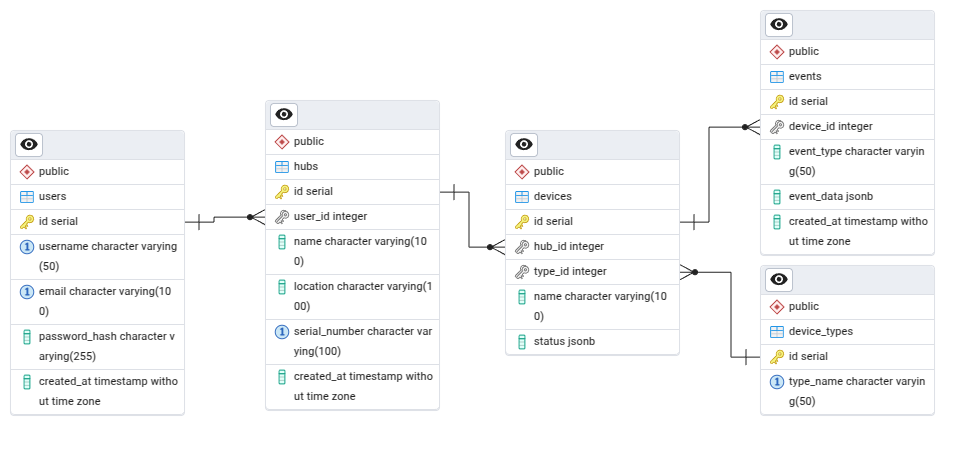
\includegraphics[width=0.95\textwidth]{pics/erd_lab1.png}
  \caption*{Рисунок 1 - ER-диаграмма.}
\end{figure}

\section*{Тема БД: <<Система управления умным домом>>}
База данных предназначена для хранения информации о пользователях, хабах и устройствах умного дома, а также событий, которые генерируют эти устройства. Она обеспечивает:
\begin{itemize}
  \item[$-$] регистрацию и управление пользователями;
  \item[$-$] хранение информации о хабах и их местоположении;
  \item[$-$] классификацию устройств по типам и отслеживание их состояния;
  \item[$-$] фиксацию событий устройств для мониторинга и анализа.
\end{itemize}

\section*{Краткое описание таблиц}
\begin{enumerate}
  \item Таблица \textbf{users}:\\
        Содержит информацию о пользователях системы.
        \begin{itemize}
          \item[$-$] \textbf{id} - уникальный идентификатор пользователя.
          \item[$-$] \textbf{username} - уникальный логин пользователя.
          \item[$-$] \textbf{email} - уникальная электронная почта.
          \item[$-$] \textbf{password\_hash} - хэш пароля.
          \item[$-$] \textbf{created\_at} - дата и время создания записи.
        \end{itemize}

  \item Таблица \textbf{hubs}:\\
        Хранит информацию о хабах, к которым подключены устройства умного дома.
        \begin{itemize}
          \item[$-$] \textbf{id} - уникальный идентификатор хаба.
          \item[$-$] \textbf{user\_id} - владелец хаба (связь с таблицей users).
          \item[$-$] \textbf{name} - название хаба.
          \item[$-$] \textbf{location} - местоположение хаба.
          \item[$-$] \textbf{serial\_number} - уникальный серийный номер хаба.
          \item[$-$] \textbf{created\_at} - дата и время создания записи.
        \end{itemize}

  \item Таблица \textbf{device\_types}:\\
        Содержит перечень типов устройств.
        \begin{itemize}
          \item[$-$] \textbf{id} - уникальный идентификатор типа устройства.
          \item[$-$] \textbf{type\_name} - название типа устройства (например, "Лампа", "Датчик").
        \end{itemize}

  \item Таблица \textbf{devices}:\\
        Содержит информацию об устройствах, подключённых к хабам.
        \begin{itemize}
          \item[$-$] \textbf{id} - уникальный идентификатор устройства.
          \item[$-$] \textbf{hub\_id} - связь с таблицей hubs.
          \item[$-$] \textbf{type\_id} - связь с таблицей device\_types.
          \item[$-$] \textbf{name} - название устройства.
          \item[$-$] \textbf{status} - текущий статус устройства в формате JSON.
        \end{itemize}

  \item Таблица \textbf{events}:\\
        Содержит события, генерируемые устройствами.
        \begin{itemize}
          \item[$-$] \textbf{id} - уникальный идентификатор события.
          \item[$-$] \textbf{device\_id} - связь с таблицей devices.
          \item[$-$] \textbf{event\_type} - тип события (например, "включение", "изменение температуры").
          \item[$-$] \textbf{event\_data} - данные события в формате JSON.
          \item[$-$] \textbf{created\_at} - дата и время создания записи.
        \end{itemize}
\end{enumerate}


\section*{Вывод}

В ходе лабораторной работы были изучены пользователи, роли и типы данных в PostgreSQL. Была спроектирована структура базы данных для системы управления умным домом и создана соответствующая ER-диаграмма. Также выполнены SQL-скрипты для создания таблиц с ограничениями и индексами, включая таблицы пользователей, хабов, типов устройств, устройств и событий. В результате закреплены навыки проектирования и создания реляционной базы данных.
\newpage

\setminted{style = rainbow_dash, fontsize = \small} % https://pygments.org/styles/

\section*{Приложение А1. Исходный код}
\inputminted{Dockerfile}{code/Containerfile}

\section*{Приложение А2. Исходный код}
\inputminted{sql}{code/init.sql}

\end{document}
